\def\chapterfigurecaption{Inclusion Exclusion}
\def\chaptergraphic{
\newcommand{\vertexradius}{2.5pt}
\newcommand{\vertexscale}{.5}
\newcommand{\bigvertexscale}{1}
\newcommand{\vertex}{\node[circle, fill=black, scale=\vertexscale] }
\newcommand{\highlighta}{red!20}
\newcommand{\highlightb}{blue!20}
\newcommand{\highlightc}{green!20}
\newcommand{\shadinga}{gray!20}
\newcommand{\smallvertex}{\node[circle, fill=black, scale=.2]}
\newcommand{\highlightlinewidth}{3pt}

\tikzset{every path/.style={line width=1 pt}}
\begin{scope}[shift={(-5, -4.2)},scale=.2, rotate=90]
    \tikzset{every path/.style={}}
    \begin{scope}[shift={(-24,2)}]
        \draw[line width = 1pt]  (13,-3) rectangle (17,-7);
        \clip (-17:15.2947) circle[radius=1];
        \clip (-18:16.477) circle[radius=1];
        \clip (-21:15.6861) circle[radius=1];
        \fill[red!20] (-17:15.2947) circle[radius=1];
        \fill[red!20] (-18:16.477) circle[radius=1];
        \fill[red!20] (-21:15.6861) circle[radius=1];
        \draw[line width = 1pt] (-17:15.2947) circle[radius=1];
        \draw[line width = 1pt] (-18:16.477) circle[radius=1];
        \draw[line width = 1pt] (-21:15.6861) circle[radius=1];
        \end{scope}\begin{scope}[shift={(15,-3)}]
        \draw[line width = 1pt]  (-2,2) rectangle (2,-2);
        \draw[line width = 1pt] (120:0.7) circle[radius=1];
        \draw[line width = 1pt] (0:0.7) circle[radius=1];
        \draw[line width = 1pt] (240:0.7) circle[radius=1];
        \fill[red!20] (120:0.7) circle[radius=1];
        \fill[red!20] (0:0.7) circle[radius=1];
        \fill[red!20] (240:0.7) circle[radius=1];
        \draw[line width = 1pt] (120:0.7) circle[radius=1];
        \draw[line width = 1pt] (0:0.7) circle[radius=1];
        \draw[line width = 1pt] (240:0.7) circle[radius=1];
        \end{scope}\begin{scope}[shift={(7,2)}]
        \draw[line width = 1pt]  (-2,2) rectangle (2,-2);
        \clip (120:0.7) circle[radius=1];
        \draw[line width = 1pt] (0:0.7) circle[radius=1];
        \draw[line width = 1pt] (240:0.7) circle[radius=1];
        \fill[red!20] (120:0.7) circle[radius=1];
        \fill[red!20] (0:0.7) circle[radius=1];
        \fill[red!20] (240:0.7) circle[radius=1];
        \draw[line width = 1pt] (120:0.7) circle[radius=1];
        \draw[line width = 1pt] (0:0.7) circle[radius=1];
        \draw[line width = 1pt] (240:0.7) circle[radius=1];
        \end{scope}\begin{scope}[shift={(7,-3)}]
        \draw[line width = 1pt]  (-2,2) rectangle (2,-2);
        \clip (0:0.7) circle[radius=1];
        \draw[line width = 1pt] (120:0.7) circle[radius=1];
        \draw[line width = 1pt] (240:0.7) circle[radius=1];
        \fill[red!20] (120:0.7) circle[radius=1];
        \fill[red!20] (0:0.7) circle[radius=1];
        \fill[red!20] (240:0.7) circle[radius=1];
        \draw[line width = 1pt] (120:0.7) circle[radius=1];
        \draw[line width = 1pt] (0:0.7) circle[radius=1];
        \draw[line width = 1pt] (240:0.7) circle[radius=1];
        \end{scope}\begin{scope}[shift={(7,-8)}]
        \draw[line width = 1pt]  (-2,2) rectangle (2,-2);
        \clip (240:0.7) circle[radius=1];
        \draw[line width = 1pt] (120:0.7) circle[radius=1];
        \draw[line width = 1pt] (0:0.7) circle[radius=1];
        \fill[red!20] (120:0.7) circle[radius=1];
        \fill[red!20] (0:0.7) circle[radius=1];
        \fill[red!20] (240:0.7) circle[radius=1];
        \draw[line width = 1pt] (120:0.7) circle[radius=1];
        \draw[line width = 1pt] (0:0.7) circle[radius=1];
        \draw[line width = 1pt] (240:0.7) circle[radius=1];
        \end{scope}\begin{scope}[shift={(-1,2)}]
        \draw[line width = 1pt]  (-2,2) rectangle (2,-2);
        \clip (120:0.7) circle[radius=1];
        \clip (0:0.7) circle[radius=1];
        \draw[line width = 1pt] (240:0.7) circle[radius=1];
        \fill[red!20] (120:0.7) circle[radius=1];
        \fill[red!20] (0:0.7) circle[radius=1];
        \fill[red!20] (240:0.7) circle[radius=1];
        \draw[line width = 1pt] (120:0.7) circle[radius=1];
        \draw[line width = 1pt] (0:0.7) circle[radius=1];
        \draw[line width = 1pt] (240:0.7) circle[radius=1];
        \end{scope}\begin{scope}[shift={(-1,-3)}]
        \draw[line width = 1pt]  (-2,2) rectangle (2,-2);
        \clip (120:0.7) circle[radius=1];
        \clip (240:0.7) circle[radius=1];
        \draw[line width = 1pt] (0:0.7) circle[radius=1];
        \fill[red!20] (120:0.7) circle[radius=1];
        \fill[red!20] (0:0.7) circle[radius=1];
        \fill[red!20] (240:0.7) circle[radius=1];
        \draw[line width = 1pt] (120:0.7) circle[radius=1];
        \draw[line width = 1pt] (0:0.7) circle[radius=1];
        \draw[line width = 1pt] (240:0.7) circle[radius=1];
        \end{scope}\begin{scope}[shift={(-1,-8)}]
        \draw[line width = 1pt]  (-2,2) rectangle (2,-2);
        \clip (0:0.7) circle[radius=1];
        \clip (240:0.7) circle[radius=1];
        \draw[line width = 1pt] (120:0.7) circle[radius=1];
        \fill[red!20] (120:0.7) circle[radius=1];
        \fill[red!20] (0:0.7) circle[radius=1];
        \fill[red!20] (240:0.7) circle[radius=1];
        \draw[line width = 1pt] (120:0.7) circle[radius=1];
        \draw[line width = 1pt] (0:0.7) circle[radius=1];
        \draw[line width = 1pt] (240:0.7) circle[radius=1];
        \end{scope}
    
        \draw[line width = 1pt,->] (-6,-2) -- (-4,2);
        \draw[line width = 1pt,->] (-6,-3) -- (-4,-3);\draw[line width = 1pt,->] (-6,-4) -- (-4,-8) ;\draw[line width = 1pt,->](2,3) -- (4,3);\draw[line width = 1pt,->] (2,2) -- (4,-6) ;\draw[line width = 1pt,->](2,-9) -- (4,-9) ;\draw[line width = 1pt,->](2,-8) -- (4,1);\draw[line width = 1pt,->] (2,-4) -- (4,-7) ;\draw[line width = 1pt,->](2,-2) -- (4,2) ;\draw[line width = 1pt,->](10,-8) -- (12,-4);\draw[line width = 1pt,->] (10,-3) -- (12,-3) ;\draw[line width = 1pt,->](10,2) -- (12,-2);
    \end{scope}
}

\def\qed{
    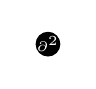
\begin{tikzpicture}[scale=.1]
    \draw[fill=black]  (0,0) ellipse (1.5 and 1.5);
        
    \node[white] at (0,0) {$\scriptscriptstyle{\partial^2}$};
    \end{tikzpicture}}

\def\chaptermark{\begin{scope}[scale=.3]
    \draw[fill=black]  (0,0) ellipse (1.5 and 1.5);
        
    \node[white] at (0,0) {$\boldsymbol {\partial^2}$};
    \end{scope}}